A brief description of the overall design of the system is presented in this section of the DD.
Our system will be developed as a 4-tiered JEE application, divided as Client Tier, Web Tier, Business Tier and the EIS Tier. It is distributed between client machines, Java EE server machine and the database.
\\The mobile and web applications in particular are thin since data operations will be computed by a central server; in this way there is no heavy load on user side clients.
\\The diagram below provides a better understanding of the components of our system, highlighting the interactions among them:
%\subsubsection{Architecture Component Diagram}
\begin{figure}[!ht]
  \centering
  \vspace{0.2cm}
  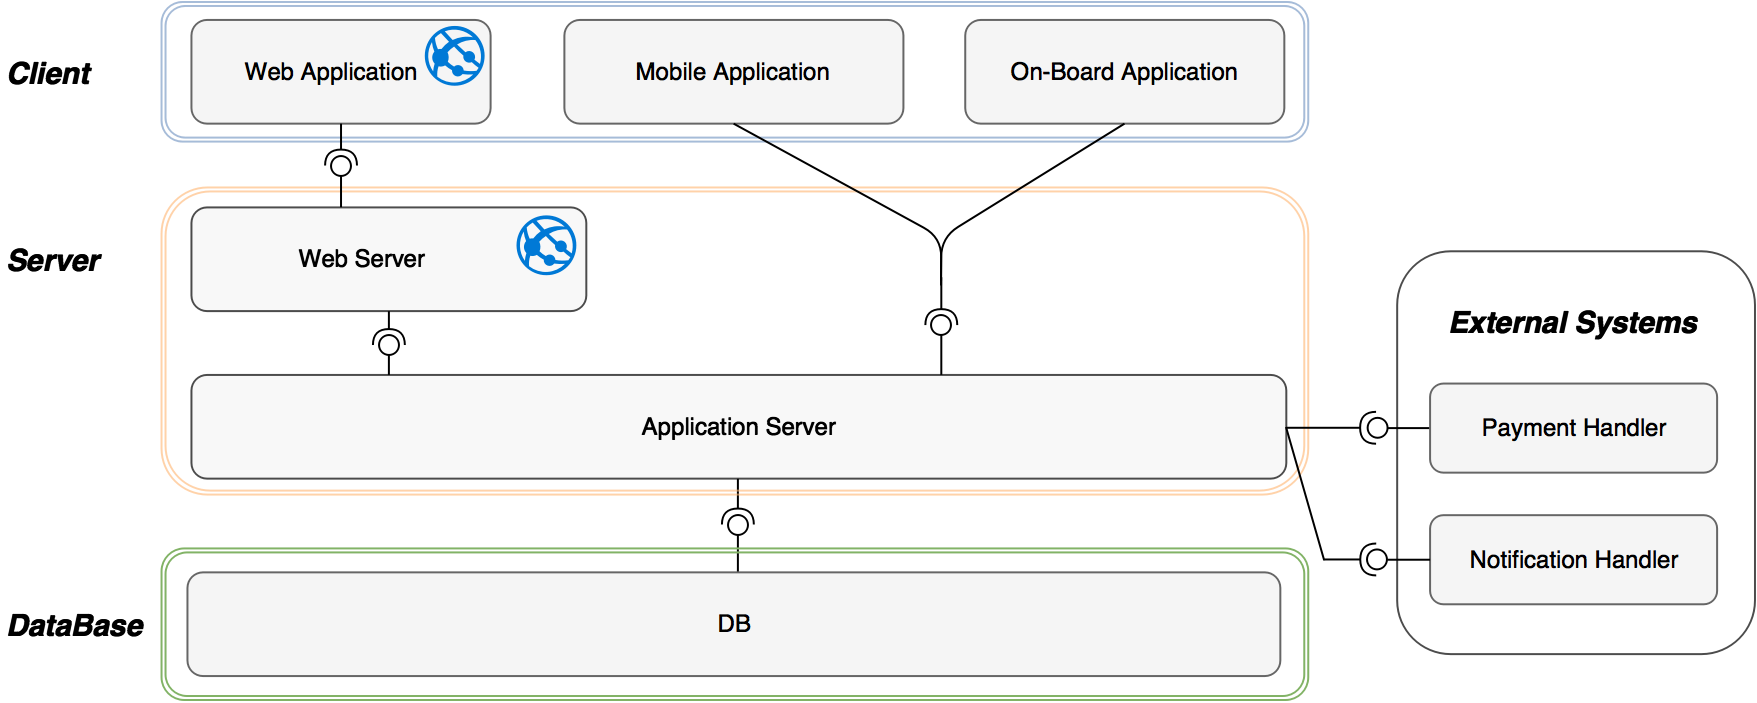
\includegraphics[width=1.0\textwidth]{/DD/architecture}\\
  \vspace{0.4cm}
  \caption{System architecture} 
  \label{fig:architecture}
\end{figure}

We can observe that the Web application needs to interact with the Web Server before accessing the Application server, the mobile application on the other side has a direct access to it.
